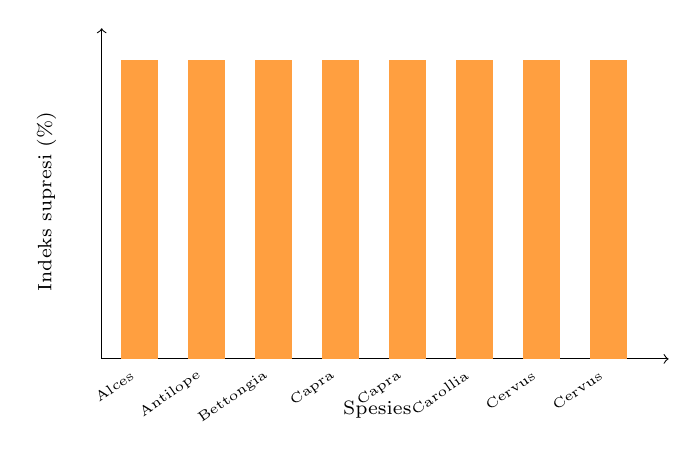
\begin{tikzpicture}[x=1cm,y=1cm]
\draw[->] (0,0) -- (7.2,0);
\draw[->] (0,0) -- (0,4.2);
\node[font=\scriptsize] at (3.5,-0.65) {Spesies};
\node[font=\scriptsize,rotate=90] at (-0.7,2) {Indeks supresi (\%)};
\fill[orange!75] (0.250,0) rectangle (0.718,3.800);
\node[font=\tiny,rotate=35,anchor=east] at (0.488,-0.12) {Alces};
\fill[orange!75] (1.100,0) rectangle (1.568,3.800);
\node[font=\tiny,rotate=35,anchor=east] at (1.338,-0.12) {Antilope};
\fill[orange!75] (1.950,0) rectangle (2.417,3.800);
\node[font=\tiny,rotate=35,anchor=east] at (2.188,-0.12) {Bettongia};
\fill[orange!75] (2.800,0) rectangle (3.268,3.800);
\node[font=\tiny,rotate=35,anchor=east] at (3.038,-0.12) {Capra};
\fill[orange!75] (3.650,0) rectangle (4.117,3.800);
\node[font=\tiny,rotate=35,anchor=east] at (3.888,-0.12) {Capra};
\fill[orange!75] (4.500,0) rectangle (4.968,3.800);
\node[font=\tiny,rotate=35,anchor=east] at (4.738,-0.12) {Carollia};
\fill[orange!75] (5.350,0) rectangle (5.817,3.800);
\node[font=\tiny,rotate=35,anchor=east] at (5.588,-0.12) {Cervus};
\fill[orange!75] (6.200,0) rectangle (6.668,3.800);
\node[font=\tiny,rotate=35,anchor=east] at (6.438,-0.12) {Cervus};
\end{tikzpicture}